\documentclass[tikz,border=2pt]{standalone}
\usepackage{amsmath,amssymb}
\usetikzlibrary{arrows.meta}
\begin{document}
% Differentiation D: P_2 -> P_1 with bases (1,t,t^2) and (1,t): taking coordinates and then multiplying
% by [D] = [[0,1,0],[0,0,2]] gives the same result as differentiating and then taking coordinates.
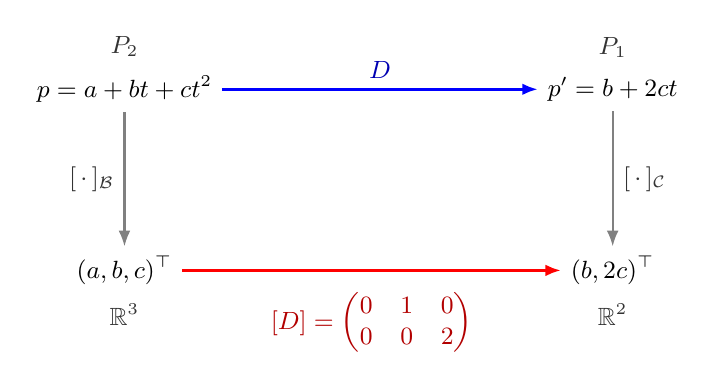
\begin{tikzpicture}[font=\small, >={Latex[length=2mm]}]
  \node (p) at (0,2.3) {$p=a+bt+ct^2$};
  \node (dp) at (6.2,2.3) {$p'=b+2ct$};
  \node (c) at (0,0) {$(a,b,c)^{\top}$};
  \node (dc) at (6.2,0) {$(b,2c)^{\top}$};
  \node[gray!40!black, anchor=south] at (p.north) {$P_2$};
  \node[gray!40!black, anchor=south] at (dp.north) {$P_1$};
  \node[gray!40!black, anchor=north] at (c.south) {$\mathbb{R}^3$};
  \node[gray!40!black, anchor=north] at (dc.south) {$\mathbb{R}^2$};
  \draw[->, blue, very thick] (p) -- (dp) node[midway, above, blue!70!black] {$D$};
  \draw[->, gray, thick] (p) -- (c) node[midway, left, gray!40!black] {$[\,\cdot\,]_{\mathcal{B}}$};
  \draw[->, gray, thick] (dp) -- (dc) node[midway, right, gray!40!black] {$[\,\cdot\,]_{\mathcal{C}}$};
  \draw[->, red, very thick] (c) -- (dc)
    node[midway, below=4pt, red!70!black] {$[D]=\begin{pmatrix}0&1&0\\0&0&2\end{pmatrix}$};
\end{tikzpicture}
\end{document}
